\documentclass{standalone}
\usepackage{tikz}
\begin{document}
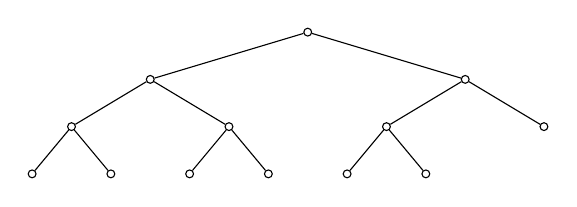
\begin{tikzpicture}[level distance=6mm,shape=circle]
  \tikzstyle{every node}=[draw,inner sep = 1pt]
  \tikzstyle{level 3}=[sibling distance=1cm]
  \tikzstyle{level 2}=[sibling distance=2cm]
  \tikzstyle{level 1}=[sibling distance=4cm]
  \node{}
     child {node{}
       child {node{} child {node{}} child {node{}}}
       child {node{} child {node{}} child {node{}}}}
     child {node{}
       child {node{} child {node{}} child {node{}}}
       child {node{}}};
\end{tikzpicture}
\end{document}
%%% Local Variables: 
%%% mode: latex
%%% TeX-master: t
%%% End: 
